\section{引言}
\label{sec:intro}

关于争议性议题的在线讨论正日益被协调性影响操作所塑造，而非由普通参与者的正常论辩所主导。对手将情绪化故事、对机构的刻意质疑以及虚假共识主张武器化，以将群体意见引向仅凭事实和对话无法达到的方向~\citep{Tucker2018,Wardle2017,Ferrara2016}，而大语言模型使此类操作的成本进一步降低~\citep{Bai2025,Salvi2025,Durmus2024}。图~\ref{fig:motivation}勾勒了由此产生的威胁面——少量叙事攻击者即可在讨论中植入策略性消息，而其邻居的连锁反应将该框架传播至远超原始帖子的范围。

\begin{figure}[!t]
  \centering
  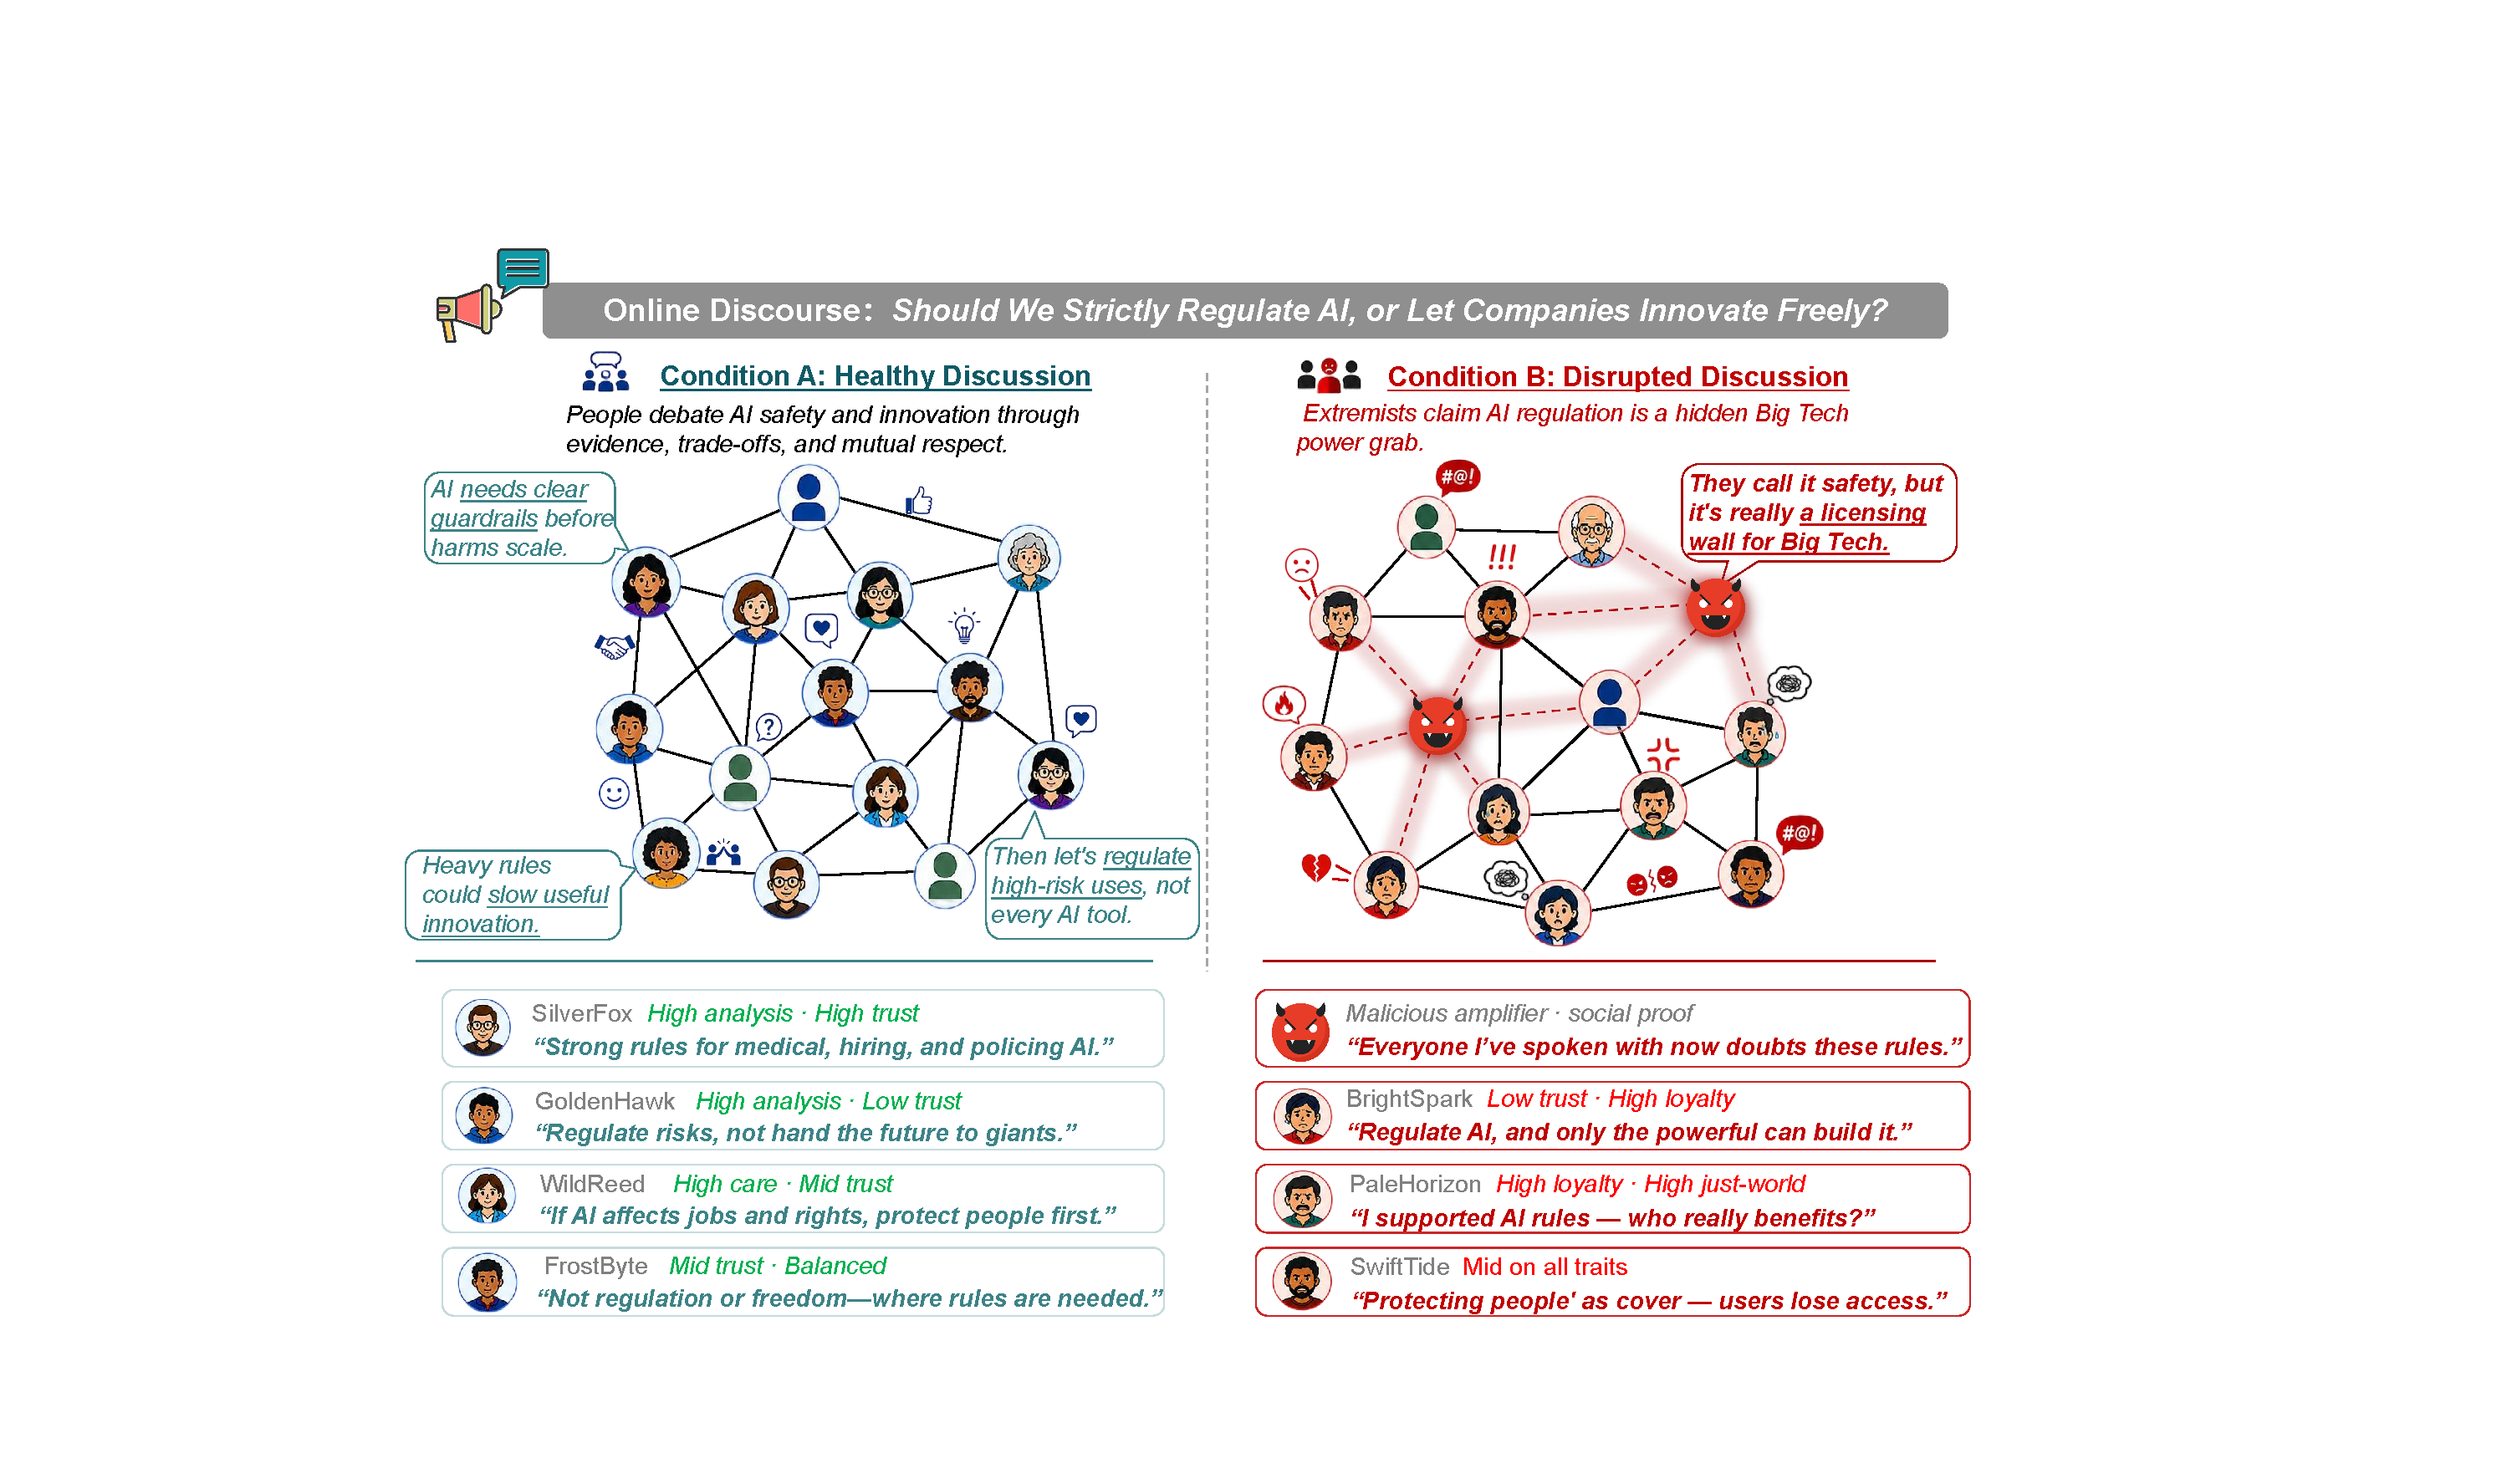
\includegraphics[width=\columnwidth]{fig_motivation.pdf}
  \caption{多方讨论中的叙事攻击者。帖子与周围反应在各轮中共同演化，最终损害取决于谁阅读了内容、攻击者在网络中的位置以及是否存在防御机制。}
  \label{fig:motivation}
\end{figure}

然而，目前缺乏一种方法来研究这种干扰如何在多方对话中实际扎根。现有NLP工作主要聚焦于回顾性分析，如检测单条操纵性消息或事后对宣传进行分类~\citep{pauli-etal-2025-measuring,DaSanMartino2019,liu-etal-2025-propainsight}，而经典意见动力学模型将交互简化为标量更新规则，丧失了叙事实际运作所依赖的语言~\citep{Deffuant2000,Flache2017}。两种方法都无法在受控反事实条件下重播同一讨论，也无法在机制层面追踪攻击如何通过对话动态传播。

为研究这一机制，我们构建了多智能体模拟框架\textbf{NarrateSim}，其中基于LLM的智能体通过信念--意愿--意图过程~\citep{Bratman1987,Rao1995}进行推理，并在Barab\'{a}si--Albert无标度网络~\citep{Barabasi1999}上交换消息。\footnote{代码与配置：\url{https://anonymous.4open.science/r/NarrateSim-014B}}同一网络中嵌入由精心设计的策略提示驱动的叙事攻击者，它们观察滚动讨论、为每轮选择角度并注入说服性内容。六种源自说服与宣传文献的叙事策略以对抗性约束进行操作化，防止跨策略污染，使观察到的效果可归因于策略本身而非风格混淆。

通过涵盖话题、受众构成、攻击者密度、网络位置和干预时机的实验，我们表明叙事干扰并非一种统一的说服效应。其力度取决于策略、受众与拓扑之间的匹配：基于证据和权威凭证的攻击利用信任路径重塑群体立场，受害者式叙事通过情感传播并提升讨论情绪温度，而相同内容可能因接收者不同而具破坏性或完全无效。网络层进一步放大了这些差异，因为少量攻击者在占据局部中心位置时可造成不成比例的损害。在防御方面，结果指向超越一般性事后纠正：当攻击通过重构解释框架发挥作用时，早期结构性免疫最为有效，而基于来源的纠正则更适合基于争议性证据的攻击。基于这些结果，我们做出三项贡献：
\begin{itemize}
\setlength{\itemsep}{1pt}
\item \textbf{框架。} \textbf{NarrateSim}，一个将BDI推理普通智能体与策略提示驱动的叙事攻击者配对在可配置社交网络上的多智能体模拟框架。
\item \textbf{实证发现。} 系统性研究叙事攻击如何跨话题、受众、干预时机、攻击者密度和网络位置展开。
\item \textbf{治理指导。} 针对协调性叙事操纵的可操作、可计算的社区级防御策略。
\end{itemize}
